
\begin{frame}
\frametitle{3. ~ Conformal maps}

A \emph{\bfseries conformal map} between two regions of the plane is a transformation that preserves shapes infinitesimally.
More precisely: it preserves angles.

\bigskip
\pause

\begin{center}
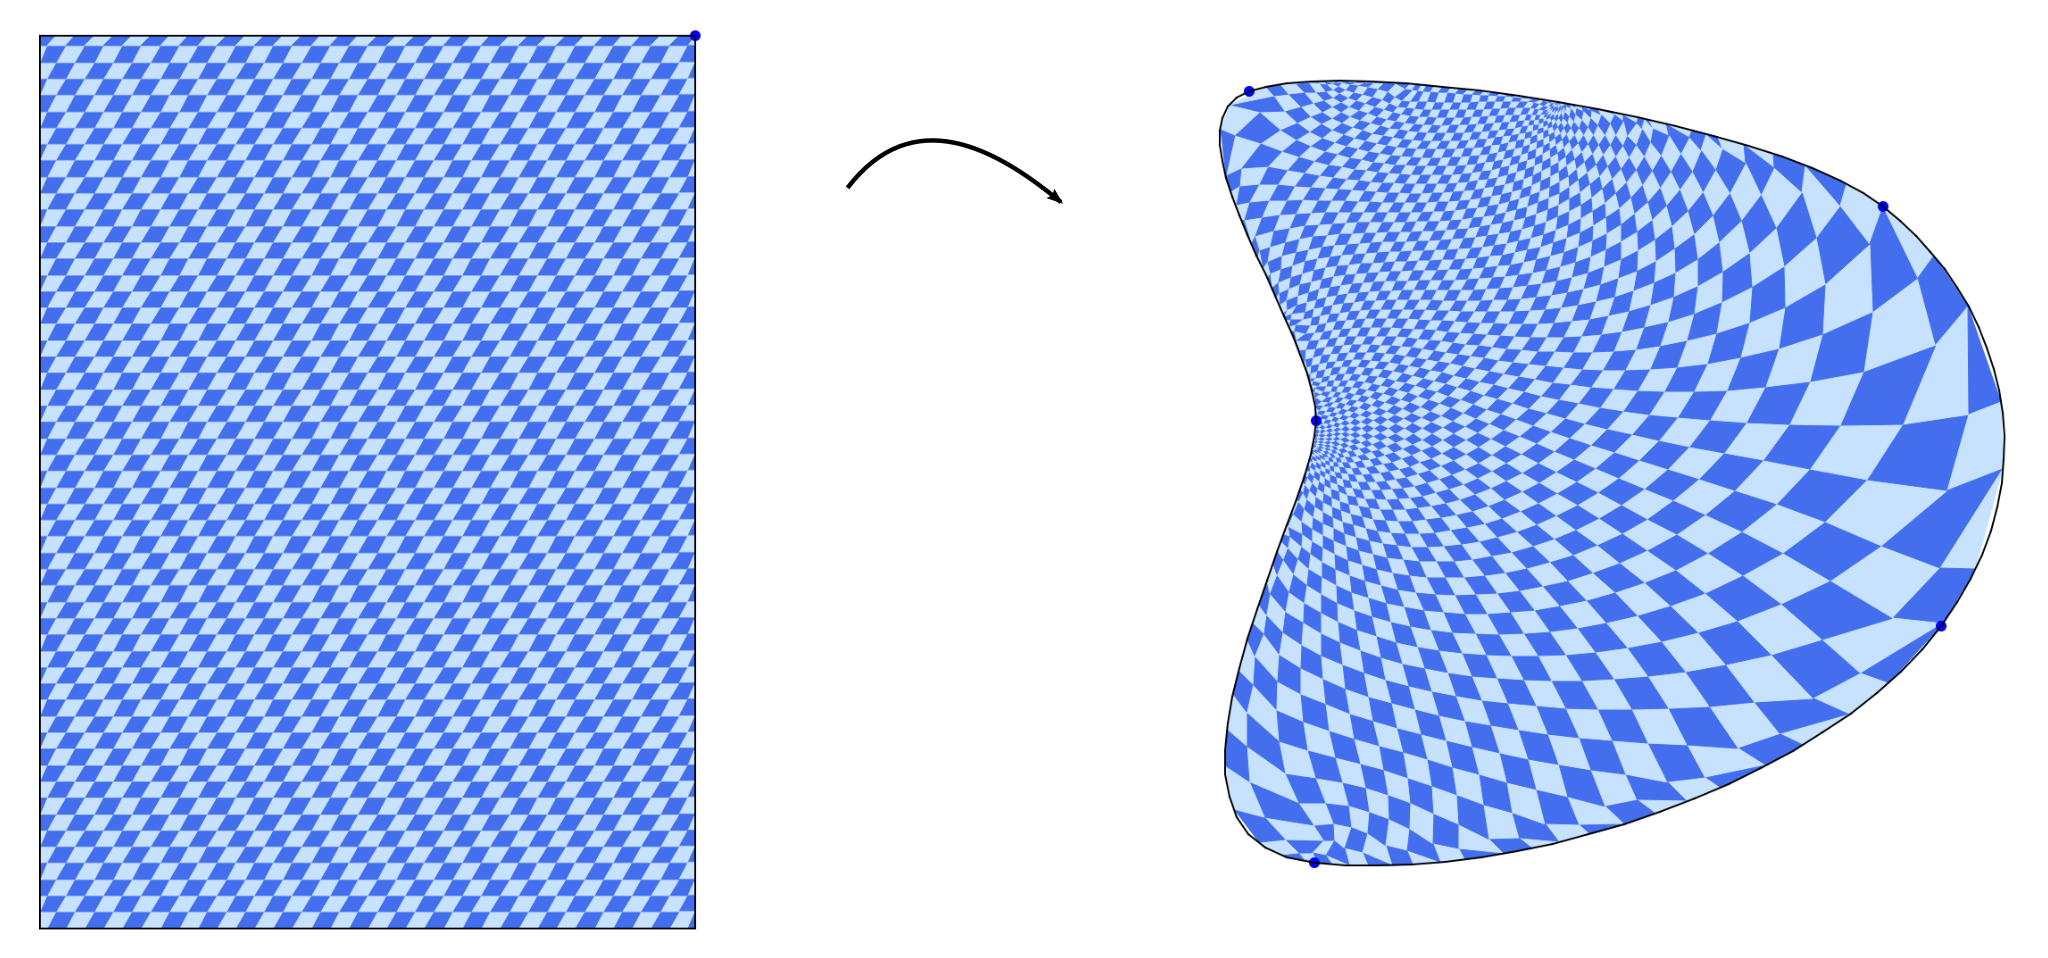
\includegraphics[width=\textwidth]{Conf1.pdf}
\end{center}

\end{frame}




\begin{frame}
\frametitle{3. ~ Conformal maps}

Conformal maps are intensely studied by mathematicians and have many important real-world applications

\bigskip
\pause

\begin{center}
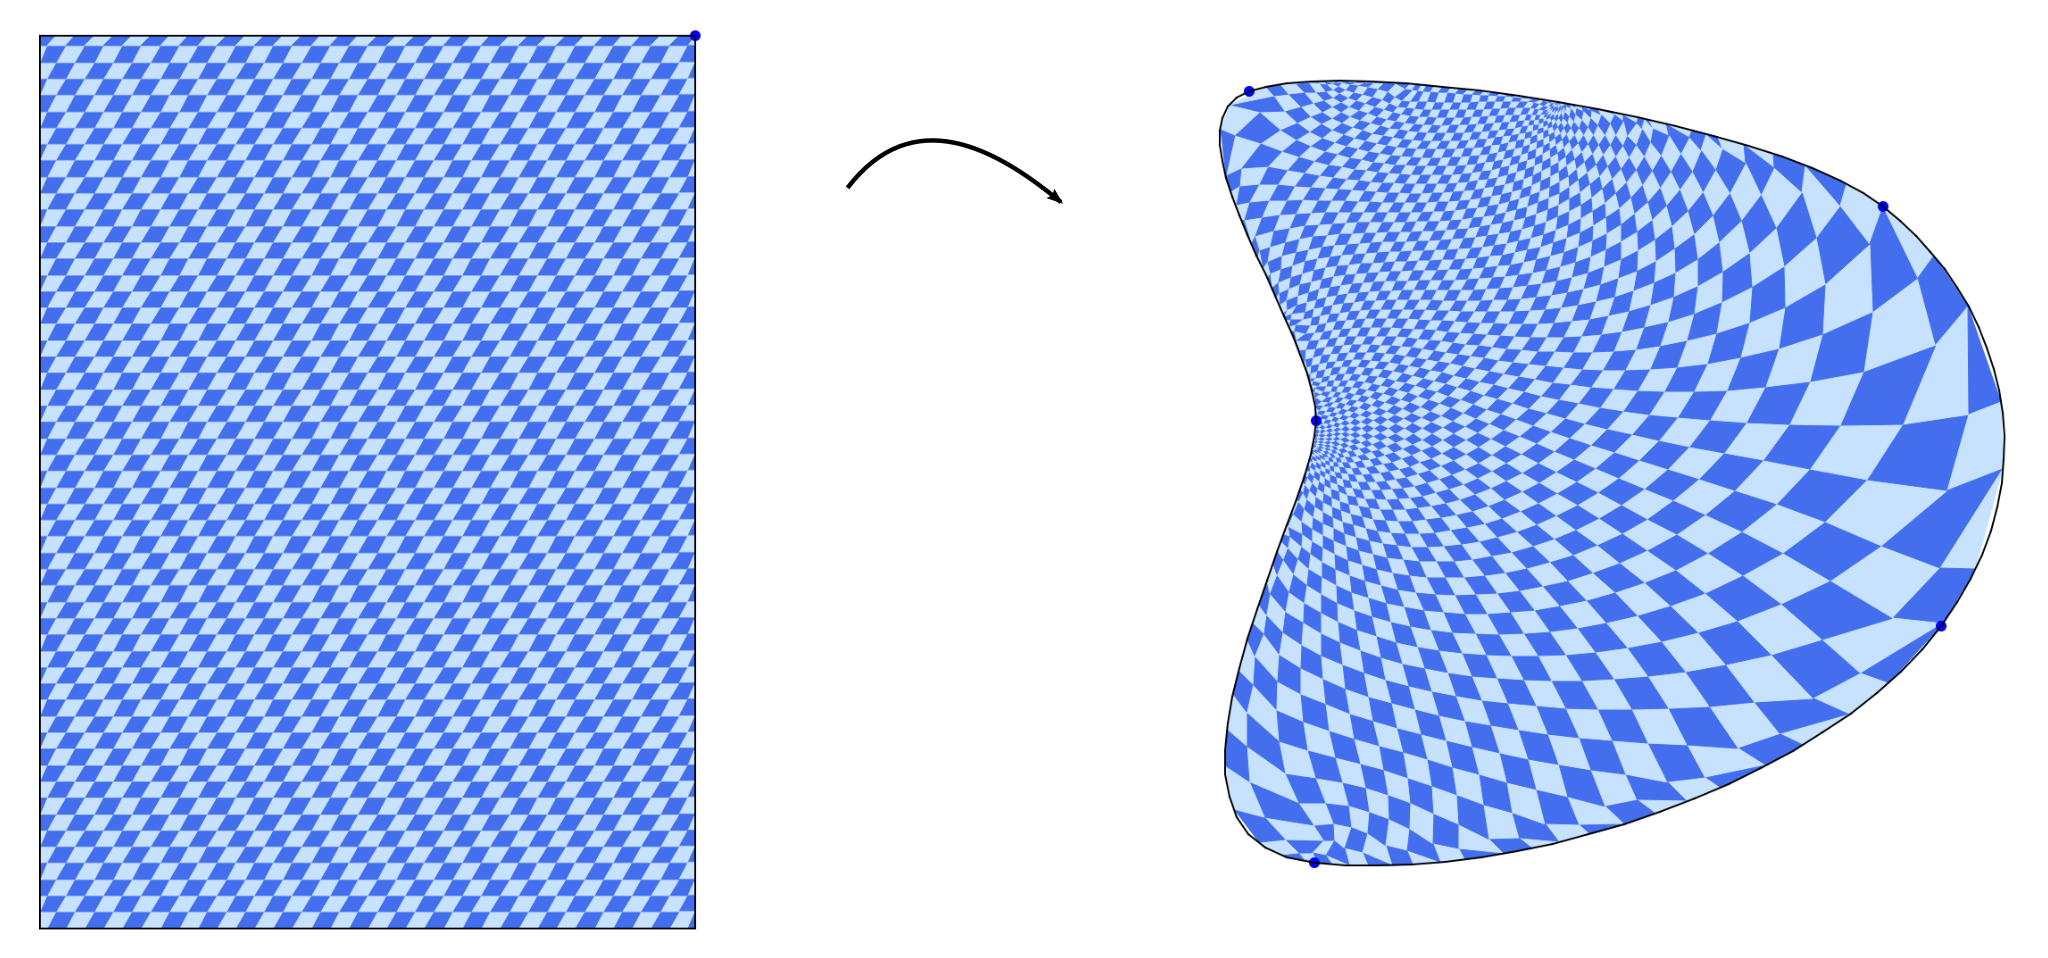
\includegraphics[width=\textwidth]{Conf1.pdf}
\end{center}

\end{frame}